\  
\
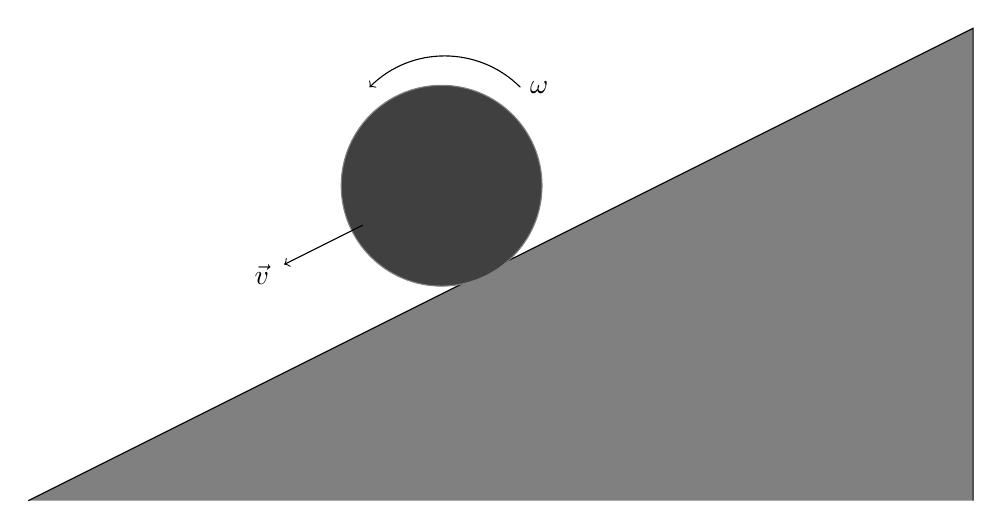
\begin{tikzpicture}
\filldraw[fill=gray, draw = black] (0,0) -- (12,6)--(12,0);
\filldraw[fill=darkgray, draw=gray] (5.25,4) circle (1.275cm);
\draw[->] (6.25,5.25) arc (45:135:1.355cm);
\draw (6.25,5.25) node[anchor=west] {$\omega$};
\draw[->] (4.25,3.5) -- (3.25,3);
\draw (2.75,2.875) node[anchor=west] {$\vec{v}$};
\end{tikzpicture}
\begin{center}
(Figure 6.7.1)
\end{center}
\
Rotational kinetic energy is the kinetic energy that objects get from spinning. The formula for rotational kinetic energy is akin to the formula for linear kinetic energy so I will just give it to you. \begin{equation}K_{rotational}=\frac{I\omega^2}{2}\end{equation} We can think of $I$ as being the mass and $\omega$ as being the velocity. This formula should match all of our intuitions. We will use it most often when considering objects that are rolling, that is, when objects are both rotating and moving linearly. In this case , when we want to use conservation of energy, we have to consider both the rotational kinetic energy and the linear kinetic energy, in some cases, we will just have to consider the rotational kinetic energy, if for example, a rotating disk is used to store energy in a car when it brakes and then power the car after. This is one reason why Tesla cars can be so efficient.